\documentclass{article}
\usepackage[margin=3.5cm]{geometry}   
\usepackage{tikz,amsmath}
\usepackage{pgfgantt}
\usetikzlibrary{arrows,shapes,positioning,shadows,trees}
\usepackage[
  colorlinks=true,
  urlcolor=cyan!70!black
  ]{hyperref}
	
\title{Homework II}
\author{Gregory Williams\\GW4975\\EE 382C Program Management}
\date{10/09/2015}

\begin{document}
	\maketitle
	\section*{Problem 9.14}
	
	\begin{center}
	\makebox[\textwidth]{
		
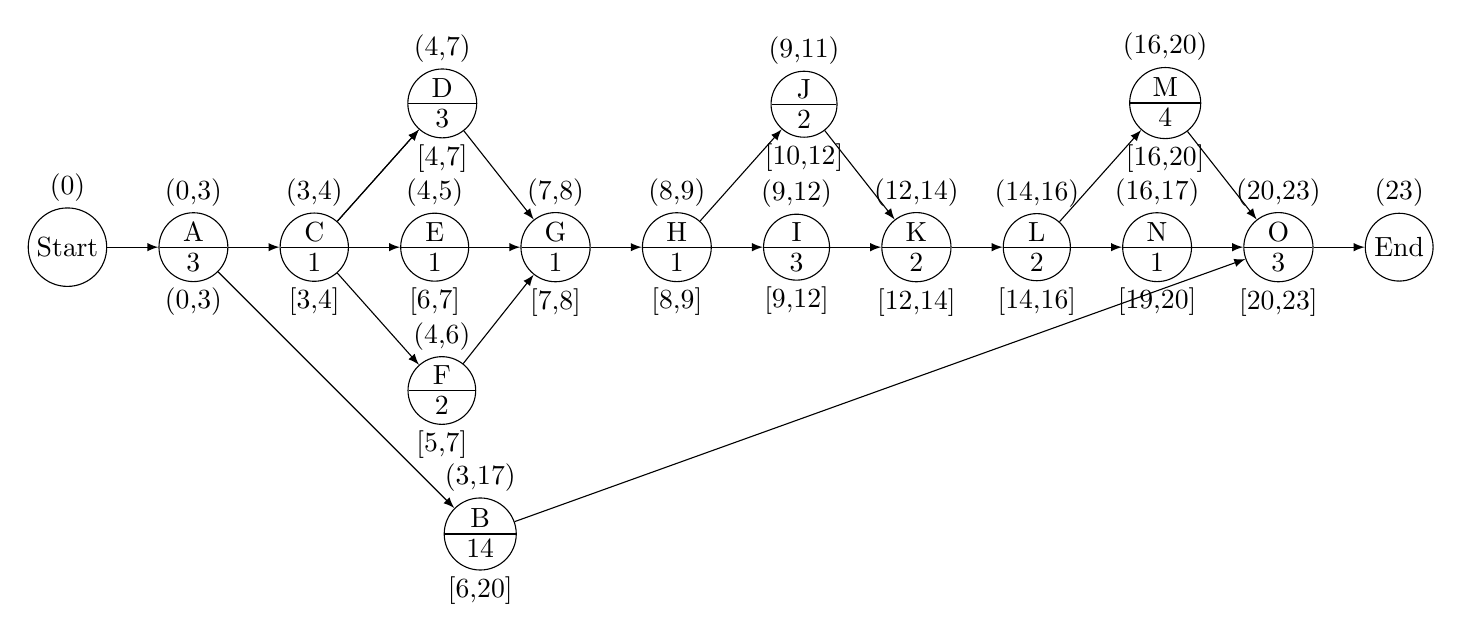
\begin{tikzpicture}[
  >=latex,
  every node/.style={draw,inner sep=2pt,minimum size=1pt},
  scale=0.5,
  node distance=.65cm,
  ]
  \node[circle, label=90:(0),] (S){Start};
  \node[circle split, right = of S, label=90:{(0,3)}, label=270:{(0,3)}] (A) {A \nodepart{lower} 3};
  \node[circle split, below right = 3 and 3 of A, label=90:{(3,17)}, label=270:{[6,20]}] (B) {B \nodepart{lower} 14};
  \node[circle split, right = of A, label=90:{(3,4)}, label=270:{[3,4]}] (C) {C \nodepart{lower} 1};
  \node[circle split, above right = 1.2 and 1 of C, label=90:{(4,7)}, label=270:{[4,7]}] (D) {D \nodepart{lower} 3};
  \node[circle split, right = of C, label=90:{(4,5)}, label=270:{[6,7]}] (E) {E \nodepart{lower} 1};
  \node[circle split, below right = 1.2 and 1 of C, label=90:{(4,6)}, label=270:{[5,7]}] (F) {F \nodepart{lower} 2};
  \node[circle split, right = of E, label=90:{(7,8)}, label=270:{[7,8]}] (G) {G \nodepart{lower} 1};
  \node[circle split, right = of G, label=90:{(8,9)}, label=270:{[8,9]}] (H) {H \nodepart{lower} 1};
  \node[circle split, right = of H, label=90:{(9,12)}, label=270:{[9,12]}] (I) {I \nodepart{lower} 3};
  \node[circle split, above right = 1.2 and 1 of H, label=90:{(9,11)}, label=270:{[10,12]}] (J) {J \nodepart{lower} 2};
  \node[circle split, right = of I, label=90:{(12,14)}, label=270:{[12,14]}] (K) {K \nodepart{lower} 2};
  \node[circle split, right = of K, label=90:{(14,16)}, label=270:{[14,16]}] (L) {L \nodepart{lower} 2};
  \node[circle split, above right = 1.2 and 1 of L, label=90:{(16,20)}, label=270:{[16,20]}] (M) {M \nodepart{lower} 4};
  \node[circle split, right = of L, label=90:{(16,17)}, label=270:{[19,20]}] (N) {N \nodepart{lower} 1};
  \node[circle split, right = of N, label=90:{(20,23)}, label=270:{[20,23]}] (O) {O \nodepart{lower} 3};
  \node[circle, right = of O, label=90:{(23)}] (End) {End};
  
  
  \draw [->] (S) -- (A);
  \draw [->] (A) -- (B);
  \draw [->] (A) -- (C);
  \draw [->] (C) -- (D);
  \draw [->] (C) -- (E);
  \draw [->] (C) -- (F);
  \draw [->] (D) -- (G);
  \draw [->] (E) -- (G);
  \draw [->] (F) -- (G);
  \draw [->] (G) -- (H);
  \draw [->] (H) -- (I);
  \draw [->] (H) -- (J);
  \draw [->] (C) -- (D);
  \draw [->] (I) -- (K);
  \draw [->] (J) -- (K);
  \draw [->] (K) -- (L);
  \draw [->] (L) -- (M);
  \draw [->] (L) -- (N);
  \draw [->] (B) -- (O);
  \draw [->] (M) -- (O);
  \draw [->] (N) -- (O);
  \draw [->] (O) -- (End);
  
\end{tikzpicture}

}
	\end{center}
	Critical path: A-C-D-G-H-I-K-L-M-O \\
	Duration: 23 days
	\pagebreak
	\section*{Problem 9.15}
	
	{\renewcommand{\arraystretch}{1.2} 
	\begin{table}[h!tbp]
  		\begin{center}
    		\caption{Slacks for Buying Tom Cruise a Boat}
    		\label{tab:table1}
			
    		\begin{tabular}{lcccc}
				Activity & Total Slack Eq & Total Slack & Free Slack Eq & Total Slack\\
				& LS - ES & & Min\{ES$_{\text{Suc}}$\} - EF & \\
				\hline
      			A* & & 0 & & 0\\
      			B & 20-17= & 3 & 20-17= & 3\\
				C* && 0 && 0\\
				D* && 0 && 0\\
				E & 7-5= & 2 & 7-5= & 2\\
				F & 7-6= & 1 & 7-6= & 1\\
				G* && 0 && 0\\
				H* && 0 && 0\\
				I* && 0 && 0\\
				J & 12-11= & 1 & 12-11= & 1\\
				K* && 0 && 0\\
				L* && 0 && 0\\
				M* && 0 && 0\\
				N & 20-17= & 3 & 20-17= & 3\\
				O* && 0 && 0\\
				\hline
				\multicolumn{3}{c}{* = On the Critical Path}\\
    		\end{tabular}
  		\end{center}
	\end{table}
	}
	
	\section*{Problem 9.19}
	\subsection*{(a)}
	\begin{center}
	\makebox[\textwidth]{
		
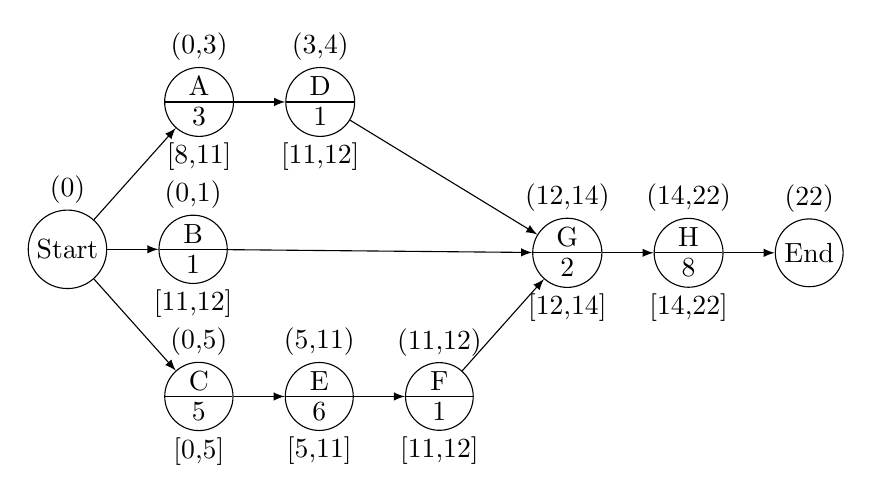
\begin{tikzpicture}[
  >=latex,
  every node/.style={draw,inner sep=2pt,minimum size=1pt},
  node distance=.65cm,
  ]
  \node[circle, label=90:(0),] (S){Start};
  \node[circle split, above right = 1.2 and 1 of S, label=90:{(0,3)}, label=270:{[8,11]}] (A) {A \nodepart{lower} 3};
  \node[circle split, right = of S, label=90:{(0,1)}, label=270:{[11,12]}] (B) {B \nodepart{lower} 1};
  \node[circle split, below right = 1.2 and 1of S, label=90:{(0,5)}, label=270:{[0,5]}] (C) {C \nodepart{lower} 5};
  \node[circle split, right = of A, label=90:{(3,4)}, label=270:{[11,12]}] (D) {D \nodepart{lower} 1};
  \node[circle split, right = of C, label=90:{(5,11)}, label=270:{[5,11]}] (E) {E \nodepart{lower} 6};
  \node[circle split, right = of E, label=90:{(11,12)}, label=270:{[11,12]}] (F) {F \nodepart{lower} 1};
  \node[circle split, above right = 1.2 and 1of F, label=90:{(12,14)}, label=270:{[12,14]}] (G) {G \nodepart{lower} 2};
  \node[circle split, right = of G, label=90:{(14,22)}, label=270:{[14,22]}] (H) {H \nodepart{lower} 8};
  \node[circle, right = of H, label=90:{(22)}] (End) {End};
  
  
  \draw [->] (S) -- (A);
  \draw [->] (S) -- (B);
  \draw [->] (S) -- (C);
  \draw [->] (A) -- (D);
  \draw [->] (C) -- (E);
  \draw [->] (E) -- (F);
  \draw [->] (B) -- (G);
  \draw [->] (D) -- (G);
  \draw [->] (F) -- (G);
  \draw [->] (G) -- (H);
  \draw [->] (H) -- (End);
  
\end{tikzpicture}

}
	\end{center}
	\pagebreak
	\subsection*{(b)}
	{\renewcommand{\arraystretch}{1.2} 
	\begin{table}[h!tbp]
  		\begin{center}
    		\caption{Slacks for Buying Tom Cruise a Boat}
    		\label{tab:table2}
			
    		\begin{tabular}{lcccc}
				Activity & Total Slack Eq & Total Slack & Free Slack Eq & Total Slack\\
				& LS - ES & & Min\{ES$_{\text{Suc}}$\} - EF & \\
				\hline
      			A & 8-0= & 8 & 3-3=& 0\\
      			B & 11-0= & 11 & 12-1= & 11\\
				C* && 0 && 0\\
				D & 11-3= & 8 & 12-4= & 8\\
				E* && 0 && 0\\
				F* && 0 && 0\\
				G* && 0 && 0\\
				H* && 0 && 0\\
				\hline
				\multicolumn{3}{c}{* = On the Critical Path}\\
    		\end{tabular}
  		\end{center}
	\end{table}
	}
	
	\noindent The total slack means that the activity may be delayed from the early start by that amount of time without affecting the total project duration; the free slack is the amount of time the activity may be delayed without delaying any other activity in the project.\\
	For this project, investigating the demand can be delayed for 8 weeks without affecting the overall project, but if it is delayed at all it will delay the conducting of the promotional cost analysis activity.\\
	The pricing strategy and the the conducting of the promotional cost analysis activities can be delayed for their total slack times without delaying any other activities, as their total slacks and free slacks are equal.
	
	\subsection*{(c)}
	Critical Path: C-E-F-G-H\\
	For this project, the design of the product must be completed before the manufacture of the prototype models. In turn, those models must be completed before the product cost analysis, final pricing analysis, and market test activities can be completed.\\
	This project appears to be dominated by the design, manufacture, and test of the product, which makes sense. Strategies and market analyses are useful, but ultimately worthless without a product to sell.
	\subsection*{(d)}
	\begin{center}
	\makebox[\textwidth]{
		
\begin{ganttchart}[vgrid,hgrid,
	bar/.append style={fill=blue!50},
	bar incomplete/.append style={fill=Maroon},
	]{1}{22}
  \gantttitle{Gantt Chart for 9.19}{22} \\
  \gantttitlelist{1,...,22}{1} \\
	\ganttbar{A}{1}{3}\\%\ganttbar{}{5}{6} \\ %LOL, just add another bar!
	\ganttbar{B}{1}{1} \\%\ganttbar[bar/.append style={fill=gray!30}]{}{4}{4} \\
	\ganttbar{C}{1}{5} \\%\ganttbar[bar/.append style={fill=gray!30}]{}{7}{7} \\
	\ganttbar{D}{4}{4} \\
	\ganttbar{E}{6}{11} \\%\ganttbar[bar/.append style={fill=white}]{}{9}{9} \\
	\ganttbar{F}{12}{12} \\
	\ganttbar{G}{13}{14} \\%\ganttbar[bar/.append style={fill=gray!30}]{}{11}{11}\\
	\ganttbar{H}{15}{22} 
\end{ganttchart}
}
	\end{center}
	
	\section*{Problem 9.20}
	\subsection*{(a)}
	
	{\renewcommand{\arraystretch}{1.2} 
	\begin{table}[h!tbp]
  		\begin{center}
    		\caption{Calculated Mean and Standard Deviation}
    		\label{tab:table3}
			
    		\begin{tabular}{lccccc}
				\hline
				&\multicolumn{3}{c}{Time estimate (weeks)} &&\\\cline{2-4}
				Activity & Optimistic & Most likely & Pessimistic & Mean & Std. Dev.\\
				\hline
				A & 1 & 3 & 4  & 2.83 & 0.5\\
				B & 1 & 1 & 2  & 1.17 & 0.17\\
				C & 4 & 5 & 9  & 5.50 & 0.83\\
				D & 1 & 1 & 1  & 1    & 0\\
				E & 4 & 6 & 12 & 6.67 & 1.33\\
				F & 1 & 1 & 2  & 1.17 & 0.17\\
				G & 1 & 2 & 3  & 2.0  & 0.33\\
				H & 6 & 8 & 10 & 8.0  & 0.67\\
				\hline
    		\end{tabular}
  		\end{center}
	\end{table}
	}
	
	\begin{center}
	\makebox[\textwidth]{
		
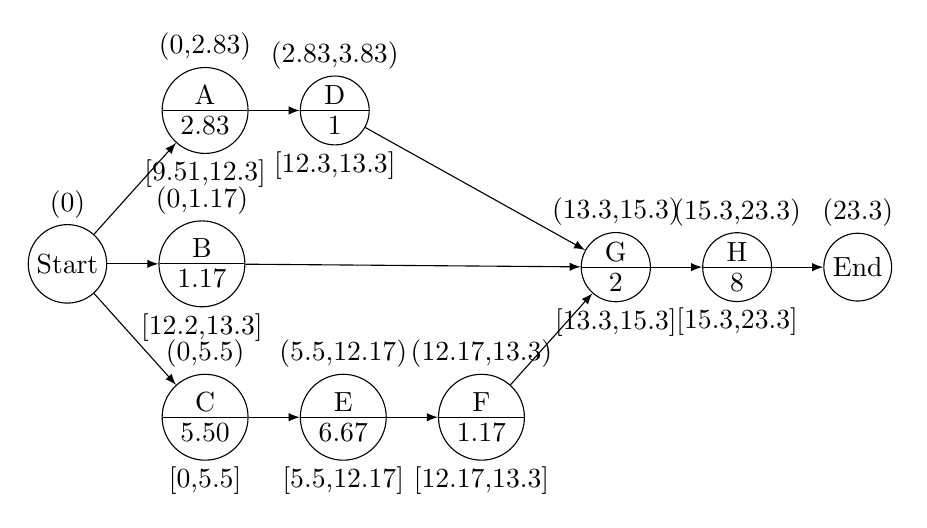
\begin{tikzpicture}[
  >=latex,
  every node/.style={draw,inner sep=2pt,minimum size=1pt},
  node distance=.65cm,
  ]
  \node[circle, label=90:(0),] (S){Start};
  \node[circle split, above right = 1.2 and 1 of S, label=90:{(0,2.83)}, label=270:{[9.51,12.3]}] (A) {A \nodepart{lower} 2.83};
  \node[circle split, right = of S, label=90:{(0,1.17)}, label=270:{[12.2,13.3]}] (B) {B \nodepart{lower} 1.17};
  \node[circle split, below right = 1.2 and 1of S, label=90:{(0,5.5)}, label=270:{[0,5.5]}] (C) {C \nodepart{lower} 5.50};
  \node[circle split, right = of A, label=90:{(2.83,3.83)}, label=270:{[12.3,13.3]}] (D) {D \nodepart{lower} 1};
  \node[circle split, right = of C, label=90:{(5.5,12.17)}, label=270:{[5.5,12.17]}] (E) {E \nodepart{lower} 6.67};
  \node[circle split, right = of E, label=90:{(12.17,13.3)}, label=270:{[12.17,13.3]}] (F) {F \nodepart{lower} 1.17};
  \node[circle split, above right = 1.2 and 1of F, label=90:{(13.3,15.3)}, label=270:{[13.3,15.3]}] (G) {G \nodepart{lower} 2};
  \node[circle split, right = of G, label=90:{(15.3,23.3)}, label=270:{[15.3,23.3]}] (H) {H \nodepart{lower} 8};
  \node[circle, right = of H, label=90:{(23.3)}] (End) {End};
  
  
  \draw [->] (S) -- (A);
  \draw [->] (S) -- (B);
  \draw [->] (S) -- (C);
  \draw [->] (A) -- (D);
  \draw [->] (C) -- (E);
  \draw [->] (E) -- (F);
  \draw [->] (B) -- (G);
  \draw [->] (D) -- (G);
  \draw [->] (F) -- (G);
  \draw [->] (G) -- (H);
  \draw [->] (H) -- (End);
  
\end{tikzpicture}

}
	\end{center}
	\subsection*{(b)}
	{\renewcommand{\arraystretch}{1.2} 
	\begin{table}[h!tbp]
  		\begin{center}
    		\caption{Slacks for Buying Tom Cruise a Boat}
    		\label{tab:table2}
			
    		\begin{tabular}{lcccc}
				Activity & Total Slack Eq & Total Slack & Free Slack Eq & Total Slack\\
				& LS - ES & & Min\{ES$_{\text{Suc}}$\} - EF & \\
				\hline
      			A & 9.51-0= & 9.51 & 2.83-2.83=& 0\\
      			B & 12.2-0= & 12.2 & 13.3-1.1= & 12.2\\
				C* && 0 && 0\\
				D & 12.3-2.83= & 9.51 & 13.3-3.83= & 9.51\\
				E* && 0 && 0\\
				F* && 0 && 0\\
				G* && 0 && 0\\
				H* && 0 && 0\\
				\hline
				\multicolumn{3}{c}{* = On the Critical Path}\\
    		\end{tabular}
  		\end{center}
	\end{table}
	}
	\subsection*{(c)}
	\noindent Critical Path: C-E-F-G-H\newline
	Critical Path Mean Duration: 23.3 weeks\newline
	Critical Path Standard Deviation: $[0.83^2 + 1.33^2 + 0.17^2 + 0.33^2 + 0.67^2]^{1/2} = 1.75$
	\newline
	
	\noindent The critical path activities have not changed, but the expected total duration has increased to 23.3 weeks from 22 weeks. 
	\subsection*{(d)}
	
	\subsubsection*{(1)}
	\begin{equation}
		P\bigg(Z\le \frac{22-23.3}{1.75}\bigg) = P(Z \le -0.743) = 1 - P(Z \le 0.743) = 1 - 0.7704 = 0.23
	\end{equation}
	\section*{Problem 9.22}
	
	\section*{Problem 9.23}
	
\end{document}